% !TEX root = proposta-qualificacao.tex
% Template UFC - Qualificação de Mestrado

\documentclass[
    a4paper,
    12pt,
    chapter=TITLE,
    section=Title,
    subsection=Title,
    oneside,
    english,
    spanish,
    brazil,
    fleqn
]{abntex2}

\input{lib/preambulo}

\setlength{\mathindent}{0pt}

%%%%%%%%%%%%%%%%%%%%%%%%%%%%%%%%%%%%%%%%%%%%%%%%%%%%%
%%                     ATENCAO                     %%
%%%%%%%%%%%%%%%%%%%%%%%%%%%%%%%%%%%%%%%%%%%%%%%%%%%%%

%\trabalhoacademico{tccgraduacao}
%\trabalhoacademico{tccespecializacao}
\trabalhoacademico{dissertacao}
%\trabalhoacademico{tese}

%%%%%%%%%%%%%%%%%%%%%%%%%%%%%%%%%%%%%%%%%%%%%%%%%%%%%

\ehqualificacao{sim}

\removerbordasdohyperlink{sim}

\cordohyperlink{nao}

%%%%%%%%%%%%%%%%%%%%%%%%%%%%%%%%%%%%%%%%%%%%%%%%%%%%%
%%         Informacao sobre a instituicao          %%
%%%%%%%%%%%%%%%%%%%%%%%%%%%%%%%%%%%%%%%%%%%%%%%%%%%%%

\ies{Universidade Federal do Ceará}
\iessigla{UFC}
\centro{Centro de Ciências}
\departamento{Departamento de Computação}

%%%%%%%%%%%%%%%%%%%%%%%%%%%%%%%%%%%%%%%%%%%%%%%%%%%%%
%%        Informacao para TCC de Graduacao         %%
%%%%%%%%%%%%%%%%%%%%%%%%%%%%%%%%%%%%%%%%%%%%%%%%%%%%%

\graduacaoem{}
\habilitacao{bacharel}

%%%%%%%%%%%%%%%%%%%%%%%%%%%%%%%%%%%%%%%%%%%%%%%%%%%%%
%%     Informacao para TCC de Especializacao       %%
%%%%%%%%%%%%%%%%%%%%%%%%%%%%%%%%%%%%%%%%%%%%%%%%%%%%%

\especializacaoem{}

%%%%%%%%%%%%%%%%%%%%%%%%%%%%%%%%%%%%%%%%%%%%%%%%%%%%%
%%         Informacao para Dissertacao             %%
%%%%%%%%%%%%%%%%%%%%%%%%%%%%%%%%%%%%%%%%%%%%%%%%%%%%%

\programamestrado{Programa de Pós-Graduação em Ciência da Computação}
\nomedomestrado{Mestrado em Ciência da Computação}
\mestreem{Ciência da Computação}
\areadeconcentracaomestrado{Ciência da Computação}

%%%%%%%%%%%%%%%%%%%%%%%%%%%%%%%%%%%%%%%%%%%%%%%%%%%%%
%%               Informação para Tese              %%
%%%%%%%%%%%%%%%%%%%%%%%%%%%%%%%%%%%%%%%%%%%%%%%%%%%%%

\programadoutorado{}
\nomedodoutorado{}
\doutorem{}
\areadeconcentracaodoutorado{}

%%%%%%%%%%%%%%%%%%%%%%%%%%%%%%%%%%%%%%%%%%%%%%%%%%%%%
%%      Informacoes relacionadas ao trabalho       %%
%%%%%%%%%%%%%%%%%%%%%%%%%%%%%%%%%%%%%%%%%%%%%%%%%%%%%

\autor{Abner Augusto Ramos Macedo Antunes de Souza}
\titulo{Sistema de Realidade Virtual para Treinamento de Segurança em Canteiro de Obras: Uma Abordagem Imersiva para Redução de Riscos}
\data{2026}
\local{Fortaleza}

\dataaprovacao{}

%%%%%%%%%%%%%%%%%%%%%%%%%%%%%%%%%%%%%%%%%%%%%%%%%%%%%
%%           Informação sobre o Orientador         %%
%%%%%%%%%%%%%%%%%%%%%%%%%%%%%%%%%%%%%%%%%%%%%%%%%%%%%

\orientador{Prof. Dr. Joaquim Bento}
\orientadories{Universidade Federal do Ceará (UFC)}
\orientadorcentro{Centro de Ciências}
\orientadorfeminino{nao}

%%%%%%%%%%%%%%%%%%%%%%%%%%%%%%%%%%%%%%%%%%%%%%%%%%%%%
%%          Informação sobre o Coorientador        %%
%%%%%%%%%%%%%%%%%%%%%%%%%%%%%%%%%%%%%%%%%%%%%%%%%%%%%

\coorientador{}
\coorientadories{}
\coorientadorcentro{}
\coorientadorfeminino{nao}

%%%%%%%%%%%%%%%%%%%%%%%%%%%%%%%%%%%%%%%%%%%%%%%%%%%%%
%%              Informação sobre a banca           %%
%%%%%%%%%%%%%%%%%%%%%%%%%%%%%%%%%%%%%%%%%%%%%%%%%%%%%

\membrodabancadois{}
\membrodabancadoiscentro{}
\membrodabancadoisies{}
\membrodabancatres{}
\membrodabancatrescentro{}
\membrodabancatresies{}
\membrodabancaquatro{}
\membrodabancaquatrocentro{}
\membrodabancaquatroies{}
\membrodabancacinco{}
\membrodabancacincocentro{}
\membrodabancacincoies{}
\membrodabancaseis{}
\membrodabancaseiscentro{}
\membrodabancaseisies{}

\begin{document}

	% Elementos pré-textuais
	\imprimircapa
	\imprimirfolhaderosto{}
	%\imprimirfichacatalografica{1-pre-textuais/ficha-catalografica}
	%\imprimirfolhadeaprovacao
	%\imprimirdedicatoria{1-pre-textuais/dedicatoria}
	%\imprimiragradecimentos{1-pre-textuais/agradecimentos}
	%\imprimirepigrafe{1-pre-textuais/epigrafe}
	\imprimirresumo{1-pre-textuais/resumo}
	%\imprimirabstract{1-pre-textuais/abstract}
	%\renewcommand*\listfigurename{Lista de Figuras}
	%\imprimirlistadeilustracoes
	\imprimirlistadetabelas
	\imprimirlistadeabreviaturasesiglas
	%\imprimirlistadesimbolos{1-pre-textuais/lista-de-simbolos}
	\imprimirsumario

	\setcounter{table}{0}

	% Elementos textuais
	\textual
	\chapter{Introdução}
\label{cap:introducao}

\section{Contexto e Problema}

O setor da construção civil no Brasil figura como um dos mais críticos em relação à segurança laboral, ocupando a 6ª posição no ranking de acidentes de trabalho típicos e a 9ª em casos de doenças profissionais ou ocupacionais, segundo dados do \gls{MTE} \cite{mte2024esocial}. Em 2023, o país registrou 2.888 mortes decorrentes de acidentes laborais e 499.955 ocorrências de acidentes típicos via sistema eSocial, com a construção liderando esse triste cenário. Em 2024, os números agravaram-se: foram 724.228 acidentes de trabalho e 3.394 óbitos, um aumento de 11,16\% em relação ao ano anterior, com a ocupação de pedreiro entre as três com maior número de mortes \cite{mte2025canpat}. Entre as principais causas estão impactos com objetos, quedas de altura, choques elétricos e soterramentos ou desmoronamentos, fatores que frequentemente estão associados à falta de equipamentos de proteção adequados, falhas na fiscalização e deficiências na formação técnica.

Restringir o recorte ao subsetor de construção de edifícios (\gls{CNAE} 4120) torna o quadro mais nítido. Esse subsetor concentra 39,6\% dos afastamentos acidentários da construção (benefício por incapacidade B91), sendo o segmento mais afetado, segundo o Observatório de Segurança e Saúde no Trabalho \cite{smartlab2024}. O perfil de lesão é dominado por fraturas, que respondem por 51,8\% dos afastamentos por capítulo da Classificação Internacional de Doenças e por 67\% das lesões por causas externas — padrão coerente com eventos de alta energia, como quedas de altura e soterramentos \cite{smartlab2024,moreira2024accidents}. As ocupações mais atingidas são servente de obras (20\%) e pedreiro (16,3\%), exatamente o público-alvo dos treinamentos de segurança em canteiro.

No âmbito regional, os dados do Ceará reforçam a urgência do problema. Em 2024, a construção civil cearense registrou 593 acidentes de trabalho e 12 óbitos, com a fratura como lesão mais frequente (135 casos) e o subsetor de construção de edifícios à frente dos registros \cite{sesifiec2024}. Enquanto os acidentes na construção recuaram no país, no Ceará houve aumento de 2,87\% em relação ao ano anterior, na contramão da tendência nacional. Servente de obras (118 casos) e pedreiro (53 casos) lideram as ocupações atingidas, confirmando localmente o perfil profissional mais exposto.

A \gls{NR}-01 \cite{brasil2024nr01}, em seu tópico 1.7, destaca a importância da capacitação contínua em \gls{SST}, exigindo atualizações periódicas para preparar os trabalhadores para os riscos ocupacionais, uma abordagem reforçada pela NR-18 \cite{brasil2025nr18}, que foca na prevenção de acidentes e na criação de ambientes seguros na construção civil, e pela NR-35 \cite{brasil2023nr35}, específica para o trabalho em altura — risco central no perfil de acidentes aqui descrito. Para atender a essas exigências, o treinamento em \gls{RV} surge como uma alternativa tecnológica que permite aos trabalhadores praticarem, de forma imersiva e segura, a identificação de riscos, o uso correto de \glspl{EPI} e \glspl{EPC} e a resposta a emergências, sem exposição a perigos reais. Essa tecnologia não só melhora a retenção do conhecimento, mas também fortalece a cultura de segurança, contribuindo para a redução de acidentes e o cumprimento das normas regulamentadoras.

\section{Objetivo Geral}

Desenvolver e validar a Fase 1 de um protótipo modular de Realidade Virtual Imersiva para treinamento de segurança em canteiros de obras, focando na identificação e mitigação de riscos relacionados a trabalhos em altura e uso de Equipamentos de Proteção Individual (EPIs), no contexto brasileiro.

\section{Hipótese/Pressuposto}

\begin{itemize}
    \item \textbf{H1 -- Eficácia do treinamento:} O treinamento em RV resulta em ganho significativo de conhecimento sobre procedimentos de segurança em trabalhos em altura e uso correto de EPIs, evidenciado pela comparação entre pré e pós-testes nos grupos experimental e controle.

    \item \textbf{H2 -- Motivação e engajamento:} O treinamento em RV promove maior motivação e engajamento dos participantes em comparação com métodos tradicionais, evidenciado pela comparação dos questionários de motivação entre os dois grupos.

    \item \textbf{H3 -- Qualidade da experiência imersiva:} O sistema de RV apresenta níveis adequados de usabilidade, conforme medido pelo \gls{SUS}, e gera sensação significativa de presença no ambiente virtual, conforme avaliado pelo \gls{IPQ}, junto ao grupo experimental.
\end{itemize}

	\chapter{Objetivos Específicos}
\label{cap:objetivos}

Os objetivos específicos organizam-se em duas frentes complementares: a construção e a validação técnica do artefato (engenharia) e a avaliação pedagógica do treinamento com usuários.

\section{Objetivos de Engenharia}

\begin{itemize}
    \item Mapear os principais riscos associados a trabalhos em altura e ao uso inadequado de EPIs em canteiros de obras brasileiros, com base nas diretrizes da NR-18 \cite{brasil2025nr18} e NR-35 \cite{brasil2023nr35}.
    \item Projetar e implementar uma arquitetura modular orientada a eventos que desacople a lógica de negócio do motor de jogo (\textit{engine}), permitindo a autoria de cenários por dados e oferecendo afordância para múltiplos domínios de treinamento.
    \item Validar tecnicamente o sistema de forma independente do motor de jogo, por meio de suíte de testes e da execução da lógica fora do \textit{engine}, evidenciando modularidade, testabilidade e resiliência a atualizações de \gls{SDK}.
\end{itemize}

\section{Objetivos de Avaliação Pedagógica}

\begin{itemize}
    \item Avaliar o ganho de conhecimento sobre procedimentos de segurança em trabalho em altura e uso de EPIs, por meio de testes aplicados antes e após a intervenção e, condicionalmente, de um teste de retenção, comparando o grupo experimental ao grupo controle submetido a método tradicional (\textbf{H1}).
    \item Avaliar a motivação e o engajamento dos participantes nas dimensões do modelo ARCS, por meio do RIMMS, comparando os dois grupos (\textbf{H2}).
    \item Avaliar a usabilidade e a sensação de presença do sistema junto ao grupo experimental, por meio do \gls{SUS} e do \gls{IPQ} (\textbf{H3}).
\end{itemize}

	\chapter{Revisão Teórica}
\label{cap:revisao}

\section{Realidade Virtual na Educação}

O estudo de \citeonline{merchant2014} realizou uma meta-análise para avaliar a eficácia da instrução baseada em realidade virtual (RV) no ensino fundamental, médio e superior. Foram analisados 67 estudos categorizados em três formatos de RV: jogos, simulações e mundos virtuais. Os resultados indicaram que todos os formatos de RV contribuíram para a melhoria dos resultados de aprendizagem, mas os jogos mostraram maior impacto em comparação com simulações e mundos virtuais \cite[p.~30]{merchant2014}. Essa vantagem foi atribuída à estrutura interativa dos jogos, que promovem maior engajamento e motivação dos alunos. Além disso, os jogos permitem estratégias de resolução de problemas e testes de hipóteses, elementos fundamentais para o aprendizado ativo.

A pesquisa também revelou que a retenção do conhecimento a longo prazo foi mais eficaz nos ambientes gamificados, enquanto o impacto das simulações e dos mundos virtuais foi mais dependente das condições de teste. Para as simulações, os melhores resultados foram observados quando utilizadas como complemento ao ensino tradicional, permitindo aos alunos praticarem conceitos previamente introduzidos. Já os mundos virtuais, apesar de proporcionarem um ambiente aberto para interação e construção de conhecimento, apresentaram menor efetividade quando medidos ao longo do tempo. O estudo destaca a importância do \textit{design} instrucional adequado para maximizar o potencial da RV na educação, enfatizando a necessidade de estratégias pedagógicas que combinem os benefícios das diferentes abordagens de aprendizado imersivo \cite[p.~37]{merchant2014}.

\section{Aplicabilidade da Realidade Virtual no Treinamento em Segurança na Construção Civil}

A utilização da Realidade Virtual (RV) no treinamento em segurança na construção civil tem sido amplamente discutida na literatura devido ao seu potencial de oferecer um ambiente imersivo e interativo para a capacitação dos trabalhadores. \citeonline[p.~9-10]{akindele2024} destacam que a RV permite uma experiência de aprendizagem envolvente e realista, contribuindo para que os trabalhadores compreendam de forma mais adequada os riscos e adotem estratégias apropriadas para lidar com diferentes situações de perigo nos canteiros de obras. Essa tecnologia permite criar ambientes simulados para identificação de riscos, treinamento operacional e educação em segurança \cite{zhou2019,wang2020,akindele2024}.

No que diz respeito à identificação de perigos, a RV permite que os trabalhadores interajam com ambientes virtuais projetados para replicar situações reais de risco. Segundo \citeonline[p.~10]{akindele2024}, estudos demonstram que a utilização da RV melhora a capacidade de identificação de riscos em relação a métodos tradicionais, como fotografias e documentação técnica, tornando a detecção mais precisa e eficaz. A tecnologia oferece um ambiente seguro para simulação de cenários de perigo, como trabalho em altura e manuseio de equipamentos, sem riscos reais \cite{li2018,sacks2019,akindele2024}. Estudos comparativos indicam que a simulação imersiva aumenta a retenção do conhecimento e a velocidade de resposta a situações de risco quando comparada a métodos convencionais, como manuais e apresentações \cite{bhoir2015,akindele2024}.

Outro aspecto abordado é o uso da RV para o treinamento de procedimentos. A tecnologia permite que os trabalhadores pratiquem atividades críticas antes de executá-las no ambiente real, reduzindo a probabilidade de erros e aumentando a eficiência \cite[p.~10]{akindele2024}. Essa abordagem é particularmente vantajosa para a preparação de respostas a situações de emergência, nas quais a rapidez e a precisão das ações podem ser determinantes para a segurança \cite{fang2016,guo2017,akindele2024}.

A RV também se mostra uma ferramenta eficaz para a educação em segurança, sendo mais envolvente que métodos tradicionais, como palestras \cite{sacks2013,guo2017}. \citeonline[p.~10]{akindele2024} ressaltam que, ao simular tarefas e situações de risco, a RV permite que os trabalhadores adquiram conhecimentos de forma intuitiva e de fácil retenção. Além disso, a interatividade e a imersão proporcionadas por essa tecnologia favorecem a retenção de informações e o desenvolvimento de boas práticas de segurança, mitigando desafios da aprendizagem passiva \cite{akindele2024}.

\subsection{Integração da RV com a Segurança do Trabalho}

\citeonline{oliveira2024} complementam essa visão, observando que, embora a RV esteja em expansão na construção civil, a \textit{integração explícita} com a segurança do trabalho ainda é limitada. Em sua revisão sistemática, apenas 25\% dos estudos abordavam diretamente a segurança. Isso sugere que, embora a RV seja usada para treinamento de forma geral, o \textit{foco específico} na segurança ainda precisa ser ampliado.

Os autores também destacam a importância da integração da RV com metodologias como o \gls{BIM}. Essa integração permite um melhor planejamento e visualização de projetos, o que contribui para a identificação proativa de riscos e a melhoria das condições de segurança nos canteiros de obras \cite[p.~12]{oliveira2024}.

\subsection{Desafios e Lacunas na Pesquisa}

Apesar das vantagens, diversos desafios e lacunas na pesquisa sobre a aplicação da RV no treinamento em segurança ainda precisam ser superados. \citeonline[p.~12-13]{akindele2024} apontam a escassez de estudos comparativos que avaliem o impacto da aprendizagem mediada por RV em relação aos métodos tradicionais. Além disso, destacam a necessidade de investigar como variáveis individuais, como experiência prévia e conhecimento sobre segurança, afetam a eficácia do treinamento virtual. Segundo os autores, é preciso investigar se ``a experiência prévia e o nível de compreensão de segurança impactam os resultados de aprendizado dentro de um ambiente virtual'' \cite[p.~13]{akindele2024}. Estudar como a carga cognitiva influencia o desempenho do treinamento em RV pode fornecer novas direções para pesquisas futuras \cite{zhao2015,lucas2018}.

Outro desafio é a personalização dos conteúdos de RV para diferentes perfis de usuários (trabalhadores, engenheiros, gestores). \citeonline{akindele2024} enfatizam que a RV deve ser adaptada às necessidades de cada grupo. Além disso, sugerem que a RV pode ter um papel importante na redução de riscos relacionados a fatores cognitivos, como distrações, mas ressaltam que essa abordagem ainda carece de investigação \cite[p.~13]{akindele2024}.

\subsection{Recomendações para Estudos Futuros}

\citeonline[p.~14]{akindele2024} recomendam estudos mais robustos, com grupos de controle, para comparar métodos de treinamento em RV. Além disso, sugerem investigar como a experiência prévia dos trabalhadores influencia a compreensão dos conceitos de segurança no ambiente virtual. Os autores afirmam que ``um método prático de teste com diversos grupos de aprendizes e uso de grupos de controle pode fornecer bons \textit{insights}'' \cite[p.~14]{akindele2024}. Estudos futuros também poderiam investigar a combinação da RV com outras tecnologias, como realidade aumentada e sensores biométricos. \citeonline{oliveira2024} enfatizam a necessidade de maior integração entre os sistemas imersivos e as \textit{normativas de segurança}, além do desenvolvimento de estratégias para viabilizar a implementação da RV de forma acessível e eficiente.

Em suma, a literatura evidencia o potencial da RV para transformar o treinamento em segurança na construção civil, mas é fundamental que estudos futuros abordem as limitações identificadas, garantindo que a tecnologia seja utilizada de maneira eficaz e adaptada às necessidades dos profissionais da construção.

\section{Métodos de Avaliação}

Com base dos artigos selecionados, é possível fazer observações de como a efetividade dessas experiências em RV foram avaliadas por outros pesquisadores:

\subsection{Abotaleb et al. (2023)}

\citeonline{abotaleb2023} avaliaram a eficácia do treinamento em RV em comparação com um método tradicional baseado no curso ``IOSH Managing Safely\textregistered''. Para isso, estudantes de engenharia foram divididos aleatoriamente em dois grupos: um que recebeu treinamento tradicional e outro que utilizou a simulação interativa de um canteiro de obras em RV. A avaliação foi realizada por meio de um teste padronizado após o treinamento, que media a capacidade dos participantes de identificar perigos e aplicar conhecimentos de segurança. Os resultados foram analisados estatisticamente usando testes de normalidade (Shapiro-Wilk), comparação de médias (teste t ou Mann-Whitney U, dependendo da distribuição dos dados) e o teste de Levene para verificar homogeneidade de variâncias. Os achados demonstraram um desempenho significativamente superior do grupo treinado com RV, e a diferença foi confirmada estatisticamente ($p = 0{,}01$), validando a efetividade do método imersivo de aprendizagem.

\subsection{Nykänen et al. (2020)}

\citeonline{nykanen2020} adotaram um ensaio controlado randomizado (\gls{RCT}) para comparar a eficácia do treinamento em RV com o treinamento tradicional baseado em palestras. Os participantes foram divididos em grupos, e diversas medidas foram coletadas antes, imediatamente após e um mês depois do treinamento. As avaliações incluíram a autoeficácia em segurança, o \textit{locus} de controle de segurança, o conhecimento sobre identificação de perigos e a motivação para comportamentos seguros. A experiência no ambiente RV foi analisada por meio de questionários que mediram presença, envolvimento, realismo e controle, além da incidência de sintomas de simulador. Dados observacionais, como padrões de movimento dentro do ambiente virtual, foram registrados e entrevistas qualitativas foram conduzidas para capturar percepções mais detalhadas. A análise estatística utilizou modelos lineares mistos generalizados (\gls{GLMM}) para examinar as diferenças entre os grupos ao longo do tempo, garantindo uma avaliação robusta da eficácia do treinamento.

\subsection{Xu e Zheng (2021)}

\citeonline{xu2021} avaliaram a efetividade do treinamento em realidade virtual (RV) para segurança em canteiros de obras através de um experimento comparativo, onde os participantes passaram tanto pelo treinamento tradicional (vídeo instrucional) quanto pelo treinamento em RV. A avaliação foi conduzida por meio de questionários antes e depois das sessões, medindo percepções sobre a plataforma RV, realismo da simulação e desconforto do simulador. Além disso, a análise do desempenho no ambiente virtual inclui métricas quantitativas, como a taxa de erro dos participantes e o Índice de Identificação de Perigo (\gls{HII}), além da observação direta do comportamento dos trabalhadores no ambiente RV. Para complementar os dados, questionários adicionais foram aplicados após a experiência em RV, incluindo a Escala de Aceitação de Van der Laan, e análises estatísticas foram conduzidas para verificar correlações entre o nível de dificuldade dos cenários e o desempenho dos participantes.

\subsection{Joshi et al. (2021)}

Na pesquisa de \citeonline{joshi2021}, a avaliação da eficácia e efetividade do treinamento em RV para segurança em canteiros de obras foi realizada por meio de um experimento comparativo entre dois grupos de participantes: um grupo que recebeu treinamento tradicional por vídeo e outro que utilizou um módulo RV interativo. A eficácia do sistema RV foi mensurada utilizando três métricas principais: \gls{SSQ} \cite{kennedy1993}, para avaliar o nível de desconforto causado pela simulação; SUS \cite{brooke1996}, para medir a usabilidade do sistema; e \gls{PQ}, para avaliar a experiência do usuário e a sensação de imersão no ambiente virtual. Já a efetividade do treinamento foi analisada com base em duas variáveis: motivação dos participantes, medida por meio de questionários comparando os dois métodos de treinamento, e ganho de conhecimento, avaliado por meio de testes aplicados antes e depois do treinamento. Análises estatísticas, como testes $t$ e qui-quadrado, foram utilizadas para verificar a significância das diferenças entre os grupos. Os resultados indicaram que o treinamento em RV gerou um maior nível de motivação nos participantes em comparação ao método tradicional, além de demonstrar potencial para melhorar a retenção de conhecimento sobre segurança no trabalho.

\section{Gaps Identificados}

Através dos artigos lidos, os problemas mais identificados foram:

\textbf{Integração insuficiente com segurança laboral:}
\begin{itemize}
    \item Apenas uma minoria dos estudos aborda explicitamente a correlação entre RV/RA e práticas de segurança, com poucos exemplos práticos de implementação em canteiros de obras reais.
\end{itemize}

\textbf{Limitações metodológicas:}
\begin{itemize}
    \item Amostras pequenas, falta de diversidade (ex.: trabalhadores experientes) e ausência de métricas quantitativas robustas comprometem a generalização dos resultados.
\end{itemize}

\textbf{Desafios na Implementação de Tecnologias de Segurança na Construção Civil:}
\begin{itemize}
    \item \textbf{Falta de Validação Prática:} Ausência de dados empíricos de longo prazo sobre a eficácia das tecnologias na redução de acidentes e custos, além de dúvidas sobre sua viabilidade econômica e adaptação a cenários complexos.
    \item \textbf{Barreiras de Comunicação e Implementação:} A falta de alinhamento entre academia e indústria resulta em tecnologias pouco adaptadas às necessidades práticas, com desafios como interoperabilidade, custos elevados e resistência à mudança em um setor pressionado por produtividade e orçamento.
    \item \textbf{Falta de Colaboração Multissetorial:} A escassez de parcerias entre pesquisadores, empresas e trabalhadores dificulta a implementação em escala real, enquanto o desconhecimento ou a falta de recursos perpetuam o uso de métodos tradicionais.
\end{itemize}

\textbf{Falta de Exemplos no Contexto Nacional:}
\begin{itemize}
    \item A NR-18 \cite{brasil2025nr18} estabelece requisitos específicos para segurança, como uso de EPIs, sinalização e prevenção de quedas. Contudo, protótipos existentes de RV (majoritariamente desenvolvidos no exterior) não incorporam esses padrões brasileiros, limitando sua aplicabilidade local. Não foi encontrado nenhum estudo que teste a eficácia de treinamentos em RV \textbf{sob as NRs}, especialmente em cenários reais de canteiros de obras brasileiros. Não há métricas claras sobre redução de acidentes ou conformidade normativa após o uso dessas ferramentas.
    \item Protótipos internacionais não consideram particularidades da construção civil brasileira, como práticas informais, diversidade de obras (desde grandes empreendimentos urbanos a construções rurais) e desafios socioeconômicos (ex.: capacitação de mão de obra menos especializada).
\end{itemize}

	\chapter{Metodologia}
\label{cap:metodologia}

\section{Desenvolvimento do Protótipo}

O desenvolvimento da Fase 1 do protótipo do sistema de treinamento em Realidade Virtual (RV) será orientado e validado por meio de consultas a especialistas em segurança do trabalho, incluindo engenheiros de segurança e instrutores de treinamentos de NR-18 \cite{brasil2025nr18} e NR-35 \cite{brasil2023nr35}, bem como representantes de empresas e entidades do setor da construção civil, como o \gls{SENAI} e o SINDUSCON-CE.

Essas consultas visam validar os principais elementos que devem ser priorizados nos cenários virtuais, considerando as principais causas de acidentes no setor, as dificuldades enfrentadas pelos instrutores na transmissão de conhecimentos e os temas de maior relevância para o público-alvo. O foco desta fase está delimitado aos riscos de quedas de altura e ao uso correto de Equipamentos de Proteção Individual (EPIs), por representarem as situações de maior impacto e maior potencial de aproveitamento das características imersivas da RV.

\section{Ferramentas Tecnológicas}

O sistema foi desenvolvido utilizando as seguintes tecnologias:

\begin{itemize}
    \item \textbf{Motor:} Unity 6 LTS (versão 6000.3.8f1)
    \item \textbf{Linguagem de Programação:} C\#
    \item \textbf{\gls{SDK} de RV:} Meta XR SDK (versão 201.0.0)
    \item \textbf{Dispositivo alvo:} Meta Quest 3, com rastreamento de mãos (\textit{hand tracking}) como modalidade primária de entrada.
\end{itemize}

\section{Estrutura dos Cenários Virtuais}

Os cenários de treinamento serão definidos a partir de consultas com especialistas em segurança do trabalho e representantes do setor da construção civil. Esta fase contempla dois cenários principais, alinhados às diretrizes da NR-18 \cite{brasil2025nr18} e NR-35 \cite{brasil2023nr35}:

\textbf{Cenário 1 -- Seleção de EPIs}

Cena introdutória na qual o usuário é recebido por um instrutor virtual e deve selecionar e equipar os EPIs adequados ao trabalho em altura que realizará em seguida. O grupo reúne cinco tarefas em modo sequencial, com limite de 270 segundos: equipar botina de segurança, luvas, óculos de proteção, capacete com jugular (exigido pela NR-35) e cinturão de segurança tipo paraquedista. A bancada apresenta, além dos itens corretos, distratores que forçam decisões fundamentadas na norma: capacete sem jugular, cinto abdominal (vedado pela NR-35 para trabalho em altura), luva de látex (inadequada para estruturas metálicas), calçado aberto (vedado pela NR-18) e colete refletivo (não pontuado). O objetivo é desenvolver o reconhecimento dos equipamentos obrigatórios antes da exposição ao cenário de risco.

\textbf{Cenário 2 -- Trabalho em Altura}

Cenário principal de inspeção de um andaime fachadeiro com irregularidades deliberadas. O grupo reúne quatro tarefas em modo de ordem livre, com limite de 300 segundos e dependência da conclusão do Cenário 1: conectar o talabarte a um ponto de ancoragem certificado (tipo A1, conforme a ABNT NBR 16325 \cite{nbr16325}), instalar guarda-corpo ausente (NR-18, item 18.15), instalar rodapé ausente (NR-18, item 18.15) e sinalizar a queda de uma rede de proteção. Caso o usuário inicie a atividade sem corrigir as irregularidades, o sistema dispara consequências --- como a queda de uma ferramenta pela borda desprotegida e uma simulação de queda por talabarte desconectado ---, cada uma registrada como violação de segurança com penalização na pontuação. \textit{Feedback} imediato é fornecido a cada ação.

O sistema prevê expansão modular para novos cenários em fases futuras, como queda de objetos, soterramentos e inspeção geral de canteiro, conforme validação com especialistas e parceiros institucionais.

\section{Amostragem e Grupos Experimentais}

A pesquisa contará com 30 participantes, divididos aleatoriamente em dois grupos:

\begin{itemize}
    \item \textbf{Grupo Experimental (RV):} Receberá o treinamento utilizando o sistema de Realidade Virtual.
    \item \textbf{Grupo Controle (Treinamento Tradicional):} Participará do treinamento por meio de vídeo instrucional com conteúdo equivalente ao apresentado no sistema de RV.
\end{itemize}

Os participantes poderão ser trabalhadores da construção civil ou estudantes da área. A alocação aleatória entre os grupos experimental e controle caracteriza o desenho como um \textbf{estudo piloto randomizado controlado}, de caráter exploratório e pioneiro no contexto brasileiro -- onde não foram identificados estudos controlados sobre RV aplicada à segurança do trabalho sob as normas regulamentadoras nacionais. Com $n = 30$, a análise prioriza a estimativa de \textbf{tamanhos de efeito} e respectivos intervalos de confiança, mais informativos que a significância isolada nesse tamanho amostral, fornecendo subsídios para o dimensionamento de pesquisas futuras com maior poder estatístico.

\section{Instrumentos de Avaliação}

Os instrumentos foram selecionados para cobrir as três hipóteses do estudo com o mínimo de sobrecarga para os participantes, garantindo viabilidade de aplicação em contexto de pesquisa piloto.

\subsection{Instrumentos aplicados a ambos os grupos}

\begin{itemize}
    \item \textbf{Teste de Conhecimento (pré e pós-teste):} Aplicado antes e imediatamente após o treinamento, mede o ganho de conhecimento sobre procedimentos de segurança em trabalhos em altura e uso correto de EPIs. As questões serão elaboradas com base nos conteúdos dos cenários desenvolvidos e validadas por especialistas em segurança do trabalho.
    \item \textbf{\textit{Reduced Instructional Materials Motivation Survey} (RIMMS):} Versão reduzida de 12 itens (três por subescala) do IMMS, baseada no modelo ARCS \cite{keller1987} e validada por \citeonline{loorbach2015}. Avalia motivação e engajamento nas dimensões de Atenção, Relevância, Confiança e Satisfação em escala Likert de cinco pontos. Será utilizada a versão traduzida e adaptada para o português brasileiro por \citeonline{cardosojunior2020}. Aplicado após o treinamento a ambos os grupos, permite comparação direta da experiência motivacional entre o método imersivo e o vídeo instrucional com menor carga de resposta em relação ao instrumento completo.
\end{itemize}

\subsection{Instrumentos aplicados exclusivamente ao grupo experimental}

\begin{itemize}
    \item \textbf{\textit{System Usability Scale} (SUS):} Instrumento padronizado para mensurar a usabilidade e aceitação do sistema pelos usuários \cite{brooke1996}. Será utilizada a versão brasileira validada por \citeonline{lourencovalentim2022}, que apresentou equivalência semântica, idiomática, conceitual e cultural com a versão original, com consistência interna de $\alpha = 0{,}76$.
    \item \textbf{\textit{iGroup Presence Questionnaire} (IPQ):} Avalia a sensação de presença e imersão no ambiente virtual \cite{schubert2001}. Será utilizada a versão portuguesa validada por \citeonline{vasconcelosraposo2016}, com adaptações lexicais mínimas para o português brasileiro.
\end{itemize}

\subsection{Teste de Retenção (condicional)}

Sujeito à viabilidade de cronograma, um teste de retenção de conhecimento equivalente ao pós-teste será aplicado entre 30 e 45 dias após o treinamento a ambos os grupos, com o objetivo de verificar a permanência do aprendizado ao longo do tempo. Caso inviável, esta etapa será declarada como limitação do estudo e recomendada para investigações futuras.

\section{Procedimento de Coleta}

A coleta de dados seguirá a seguinte sequência para ambos os grupos:

\begin{enumerate}
    \item Assinatura do \gls{TCLE}
    \item Aplicação do pré-teste de conhecimento
    \item Realização do treinamento (RV ou vídeo instrucional, conforme o grupo)
    \item Aplicação do pós-teste de conhecimento
    \item Aplicação do questionário de motivação e engajamento
    \item Aplicação do SUS e IPQ \textit{(somente grupo experimental)}
    \item Aplicação do teste de retenção \textit{(ambos os grupos, condicional)}
\end{enumerate}

\section{Avaliação Qualitativa}

Após a conclusão do treinamento, será conduzida uma análise qualitativa baseada em entrevistas semiestruturadas com os participantes do grupo experimental. Essas entrevistas terão como objetivos explorar a experiência subjetiva dos participantes, coletar percepções sobre o realismo e a utilidade do treinamento em RV, identificar pontos fortes e fracos da abordagem e obter sugestões de melhoria para fases futuras do sistema.

	\chapter{Desenvolvimento e Arquitetura do Sistema}
\label{cap:arquitetura}

O Sistema de Realidade Virtual para Treinamento de Segurança em Canteiro de Obras foi desenvolvido em Unity 6 LTS com o Meta XR SDK, para execução no Meta Quest 3 com rastreamento de mãos como modalidade primária de entrada. A arquitetura atende a dois propósitos: criar e executar cenários de treinamento baseados em situações críticas reais da construção civil e avaliar de forma sistemática o desempenho do usuário, com foco na identificação de comportamentos seguros diante dos riscos simulados.

Em vez de concentrar interação, renderização, gerência de estado e avaliação de regras nos mesmos componentes --- prática comum em protótipos de motor de jogo, mas que dificulta manutenção e evolução ---, o sistema adota uma \gls{EDA}. A lógica de domínio reside em classes C\# puras, independentes do motor (sufixo \texttt{Core}), envolvidas por adaptadores \texttt{MonoBehaviour} que fazem a ponte com a cena, seguindo o padrão \textit{ports-and-adapters}. As camadas coordenam-se por meio de eventos tipados publicados em um barramento central, sem manter referências diretas entre si. Essa separação sustenta a testabilidade, a resiliência a atualizações de \gls{SDK} e a autoria de cenários sem alteração de código, propriedades retomadas no Capítulo~\ref{cap:validacao}.

\section{Visão Geral em Camadas}

A arquitetura organiza o sistema em sete camadas conectadas por um \texttt{EventBus} tipado, que atua como espinha de comunicação (Figura~\ref{fig:arquitetura}). As camadas vão da configuração de dados, na base, à publicação de eventos, ao núcleo de domínio, à interface reativa e à saída em rede, no topo. O acoplamento ao SDK fica confinado às camadas de publicação e de adaptadores; o núcleo de domínio, o subsistema de avaliação e a interface não possuem dependências do motor.

\begin{figure}[htb]
    \centering
    \caption{Arquitetura em camadas orientada a eventos do sistema de treinamento. MB: \texttt{MonoBehaviour}.}
    \label{fig:arquitetura}
    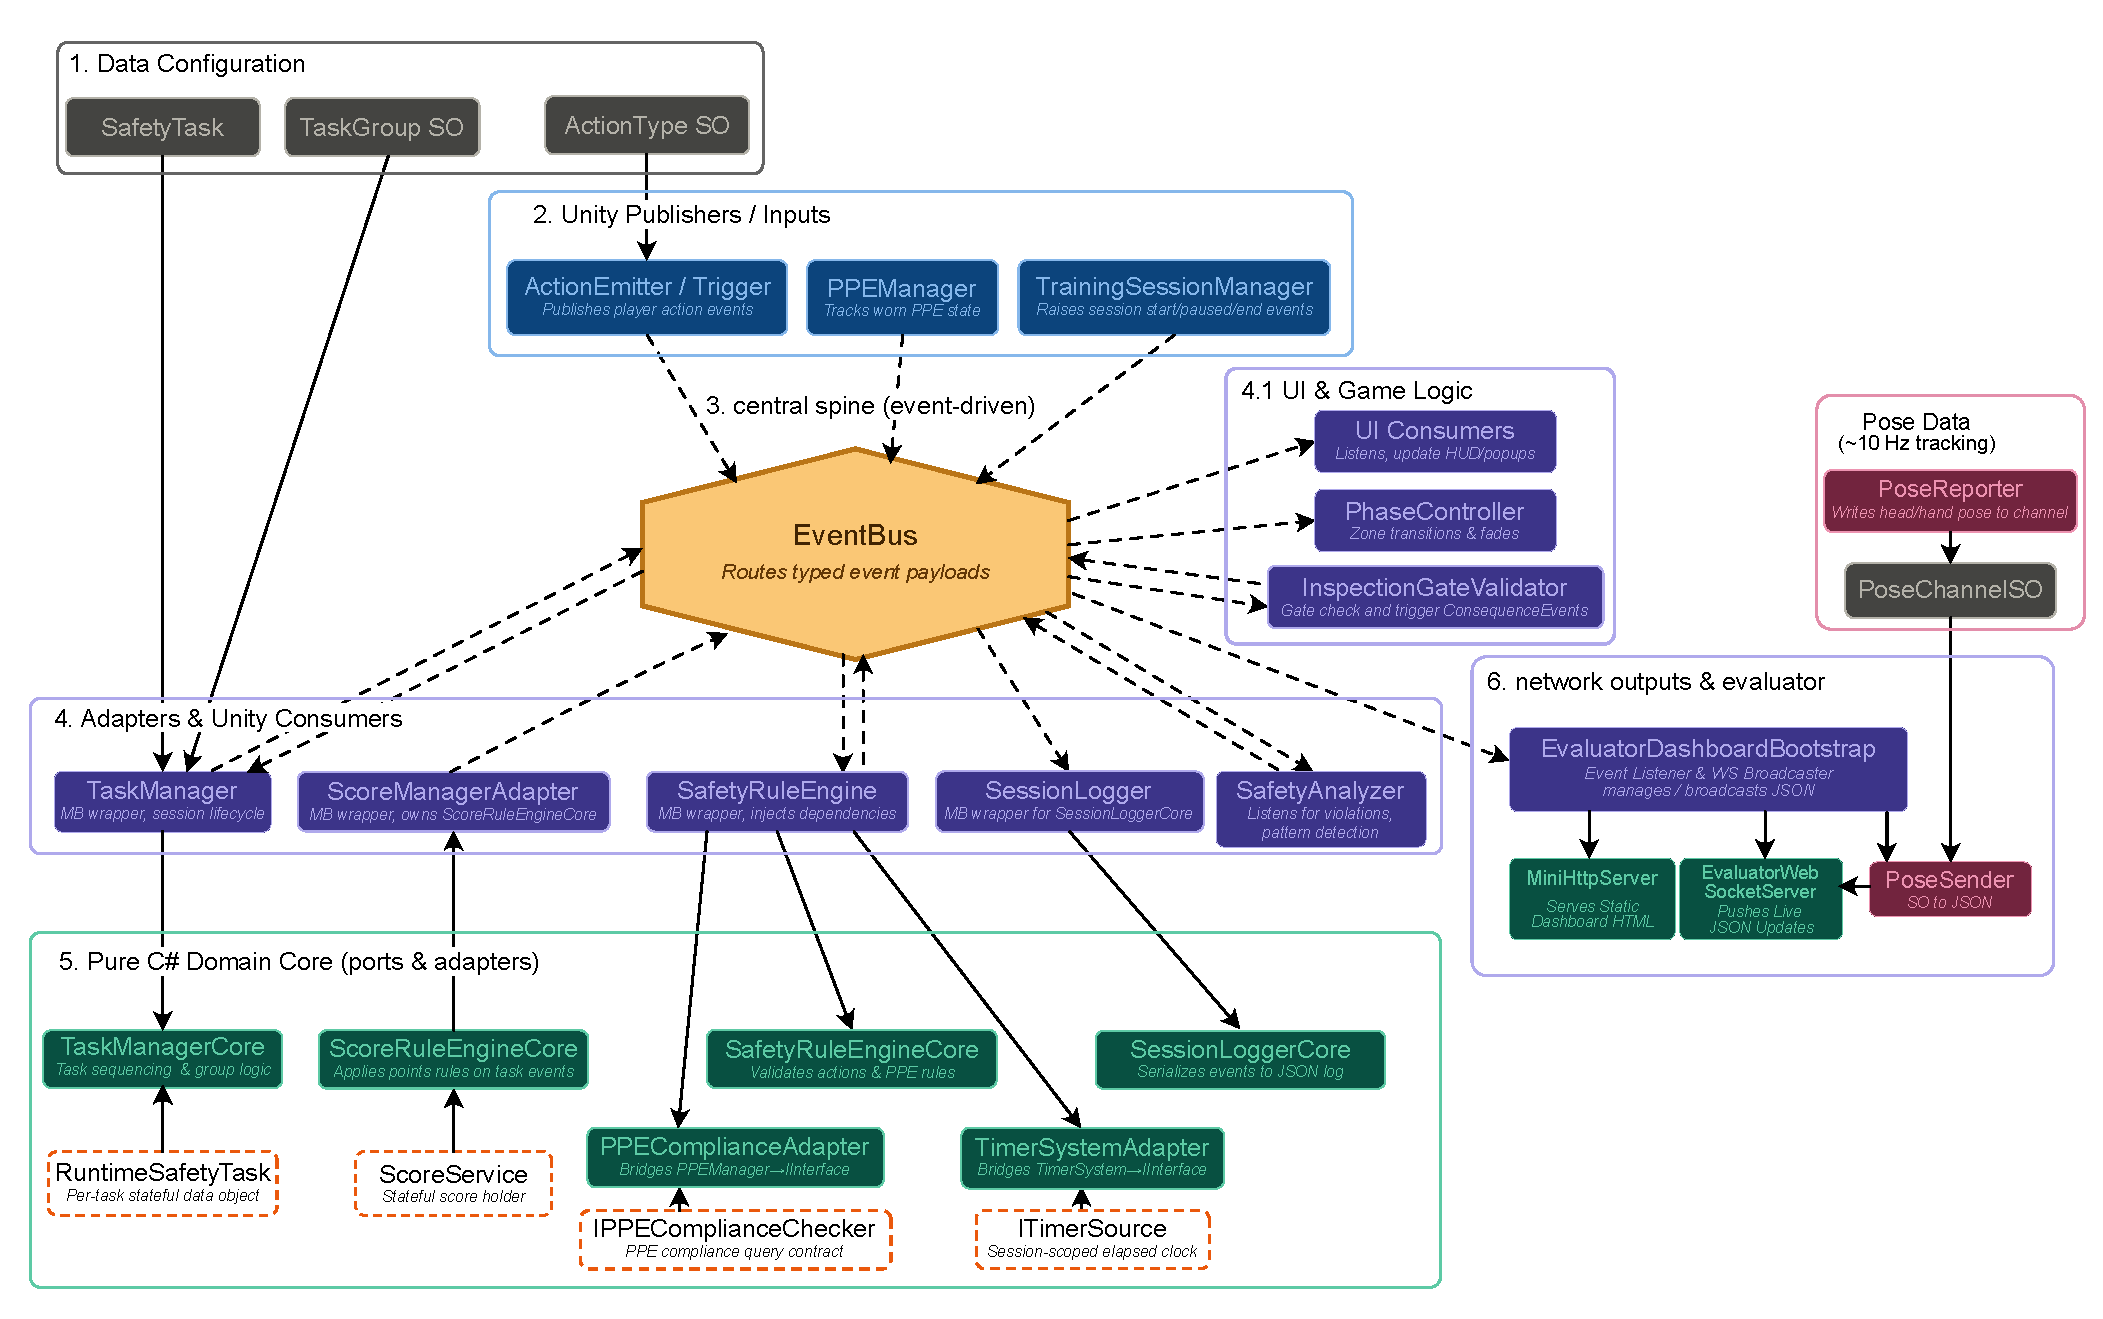
\includegraphics[width=\textwidth]{figuras/safety-proto-architecture}

    {\footnotesize Fonte: elaborado pelo autor.}
\end{figure}

\section{Camadas da Arquitetura}

\textbf{Camada 1 -- Configuração de Dados.} O conteúdo dos cenários reside em \textit{assets} nativos do editor (\texttt{ScriptableObject}), e não em código. Três tipos compõem a camada: \texttt{SafetyTask}, que descreve uma ação treinável e suas regras de pontuação; \texttt{TaskGroup}, que agrupa tarefas sob um modo de execução (sequencial ou ordem livre) e pode declarar dependências entre grupos; e \texttt{ActionType}, que define o vocabulário canônico de interações ligando objetos da cena às expectativas das tarefas. Como consequência, a autoria de cenários dispensa alteração de código e os cenários são versionados como \textit{assets}, com fluxo padrão de \textit{diff}, ramificação e revisão.

\textbf{Camada 2 -- Publicadores.} Traduz a interação física do jogador e o ciclo de vida da sessão em eventos tipados. Seus componentes são produtores puros: nunca assinam eventos. Produtores de ação emitem um evento canônico quando o jogador interage com um objeto (preensão, proximidade ou \textit{callback} do SDK de interação); o \texttt{PPEManager} publica mudanças de estado dos EPIs; e o \texttt{TrainingSessionManager} emite eventos de ciclo de sessão (início, pausa, retomada, término).

\textbf{Camada 3 -- Barramento Central.} O \texttt{EventBus} é o único \textit{broker} tipado de publicação/assinatura pelo qual fluem todas as interações entre camadas. Ele expõe primitivas genéricas de assinatura e publicação parametrizadas pelo tipo da carga do evento e processa sua fila uma vez por quadro, garantindo ordem de despacho consistente com o ciclo de atualização do motor.

\textbf{Camada 4 -- Adaptadores.} É a costura entre o motor e o núcleo independente. Cada núcleo de domínio possui um invólucro que assina o barramento, encaminha eventos para o núcleo e publica de volta os resultados. Componentes que legitimamente exigem serviços do motor --- transições de cena, esmaecimento de tela --- consomem o barramento diretamente. A injeção de dependências concentra-se aqui, e o risco de migração de SDK fica contido nesta camada e na de publicadores.

\textbf{Camada 5 -- Núcleo de Domínio (C\# puro).} É onde as principais propriedades arquiteturais são testáveis, pois suas classes não têm dependências do motor. O \texttt{TaskManagerCore} gerencia o sequenciamento de tarefas e grupos, trata dependências, \textit{timeouts} e violações de ordem nos modos sequencial e de ordem livre. O \texttt{SafetyRuleEngineCore} valida cada ação contra as tarefas ativas e verifica conformidade dos EPIs, emitindo evento de violação quando uma restrição normativa é quebrada. O \texttt{ScoreRuleEngineCore} aplica regras de pontuação e penalidade, mantendo a política de escore dentro do núcleo. O \texttt{SessionLoggerCore} assina todos os eventos do barramento e, ao final, serializa o histórico por meio de uma estratégia injetada por dependência.

\textbf{Camada 6 -- Interface do Usuário.} É puramente reativa: nenhum componente publica eventos ou mantém estado de domínio; cada um assina o barramento e apenas atualiza a exibição. As superfícies em cena incluem um HUD de pontuação, um cronômetro por tarefa, um painel de progresso de tarefa e grupo, um resumo de conclusão de sessão e avisos contextuais. Como a interface consome o mesmo protocolo de eventos das demais camadas, apresentações alternativas (um painel \textit{desktop}, uma visão de espectador) podem ser introduzidas sem alterar produtores ou núcleo de domínio.

\textbf{Camada 7 -- Saída em Rede e Painel do Avaliador.} Permite a observação remota, em tempo real, por instrutor ou pesquisador na rede local, sem intervir na simulação. Um componente de \textit{bootstrap} inicia um servidor HTTP (página estática do painel) e um servidor WebSocket (transmissão de eventos ao vivo) na inicialização do dispositivo, assina todos os eventos do barramento e os retransmite em \gls{JSON} para os navegadores conectados. Dados de pose de alta frequência (cabeça, mãos e objetos de EPI, a cerca de 10~Hz) trafegam por um canal dedicado, separado do canal de eventos discretos, para não congestioná-lo.

\section{Catálogo de Eventos}

O protótipo define 18 eventos lógicos, dos quais 16 são despachados como canais tipados do \texttt{EventBus}, implementados por 13 classes de carga (eventos correlatos compartilham uma classe distinguida por um \textit{enum} de fase). Os módulos nunca inspecionam entrada bruta nem consultam estado externo diretamente. A Tabela~\ref{tab:eventos} resume os grupos de eventos e seus principais publicadores.

\begin{table}[htb]
    \centering
    \caption{Grupos de eventos do protótipo e seus principais publicadores.}
    \label{tab:eventos}
    \begin{tabular}{lll}
        \toprule
        \textbf{Grupo} & \textbf{Eventos representativos} & \textbf{Publicador} \\
        \midrule
        Ciclo de sessão   & \texttt{SessionStarted}/\texttt{Completed} & \texttt{TrainingSessionManager} \\
        Interação         & \texttt{ActionAttempt}                     & \texttt{ActionEmitter} \\
        Conformidade EPI  & \texttt{PpeStateChanged}                   & \texttt{PPEManager} \\
        Tarefas e grupos  & \texttt{TaskStarted}/\texttt{Completed}    & \texttt{TaskManagerCore} \\
        Pontuação         & \texttt{ScoreChanged}                      & \texttt{ScoreService} \\
        Análise de risco  & \texttt{SafetyViolation}                   & \texttt{SafetyRuleEngineCore} \\
        \bottomrule
    \end{tabular}

    {\footnotesize Fonte: elaborado pelo autor.}
\end{table}

\section{Ciclo de Vida das Tarefas}

O \texttt{TaskManagerCore} avança a tarefa correspondente a cada evento de interação e publica o evento de ciclo de vida de volta no barramento. A Figura~\ref{fig:lifecycle} ilustra a máquina de estados resultante para os modos sequencial e de ordem livre: toda transição de estado é publicada como evento tipado, sem que nenhum componente mantenha referência direta ao \texttt{TaskManagerCore}.

\begin{figure}[htb]
    \centering
    \caption{Máquina de estados do ciclo de vida das tarefas nos modos sequencial e de ordem livre. Os círculos numerados traçam o caminho canônico de sucesso.}
    \label{fig:lifecycle}
    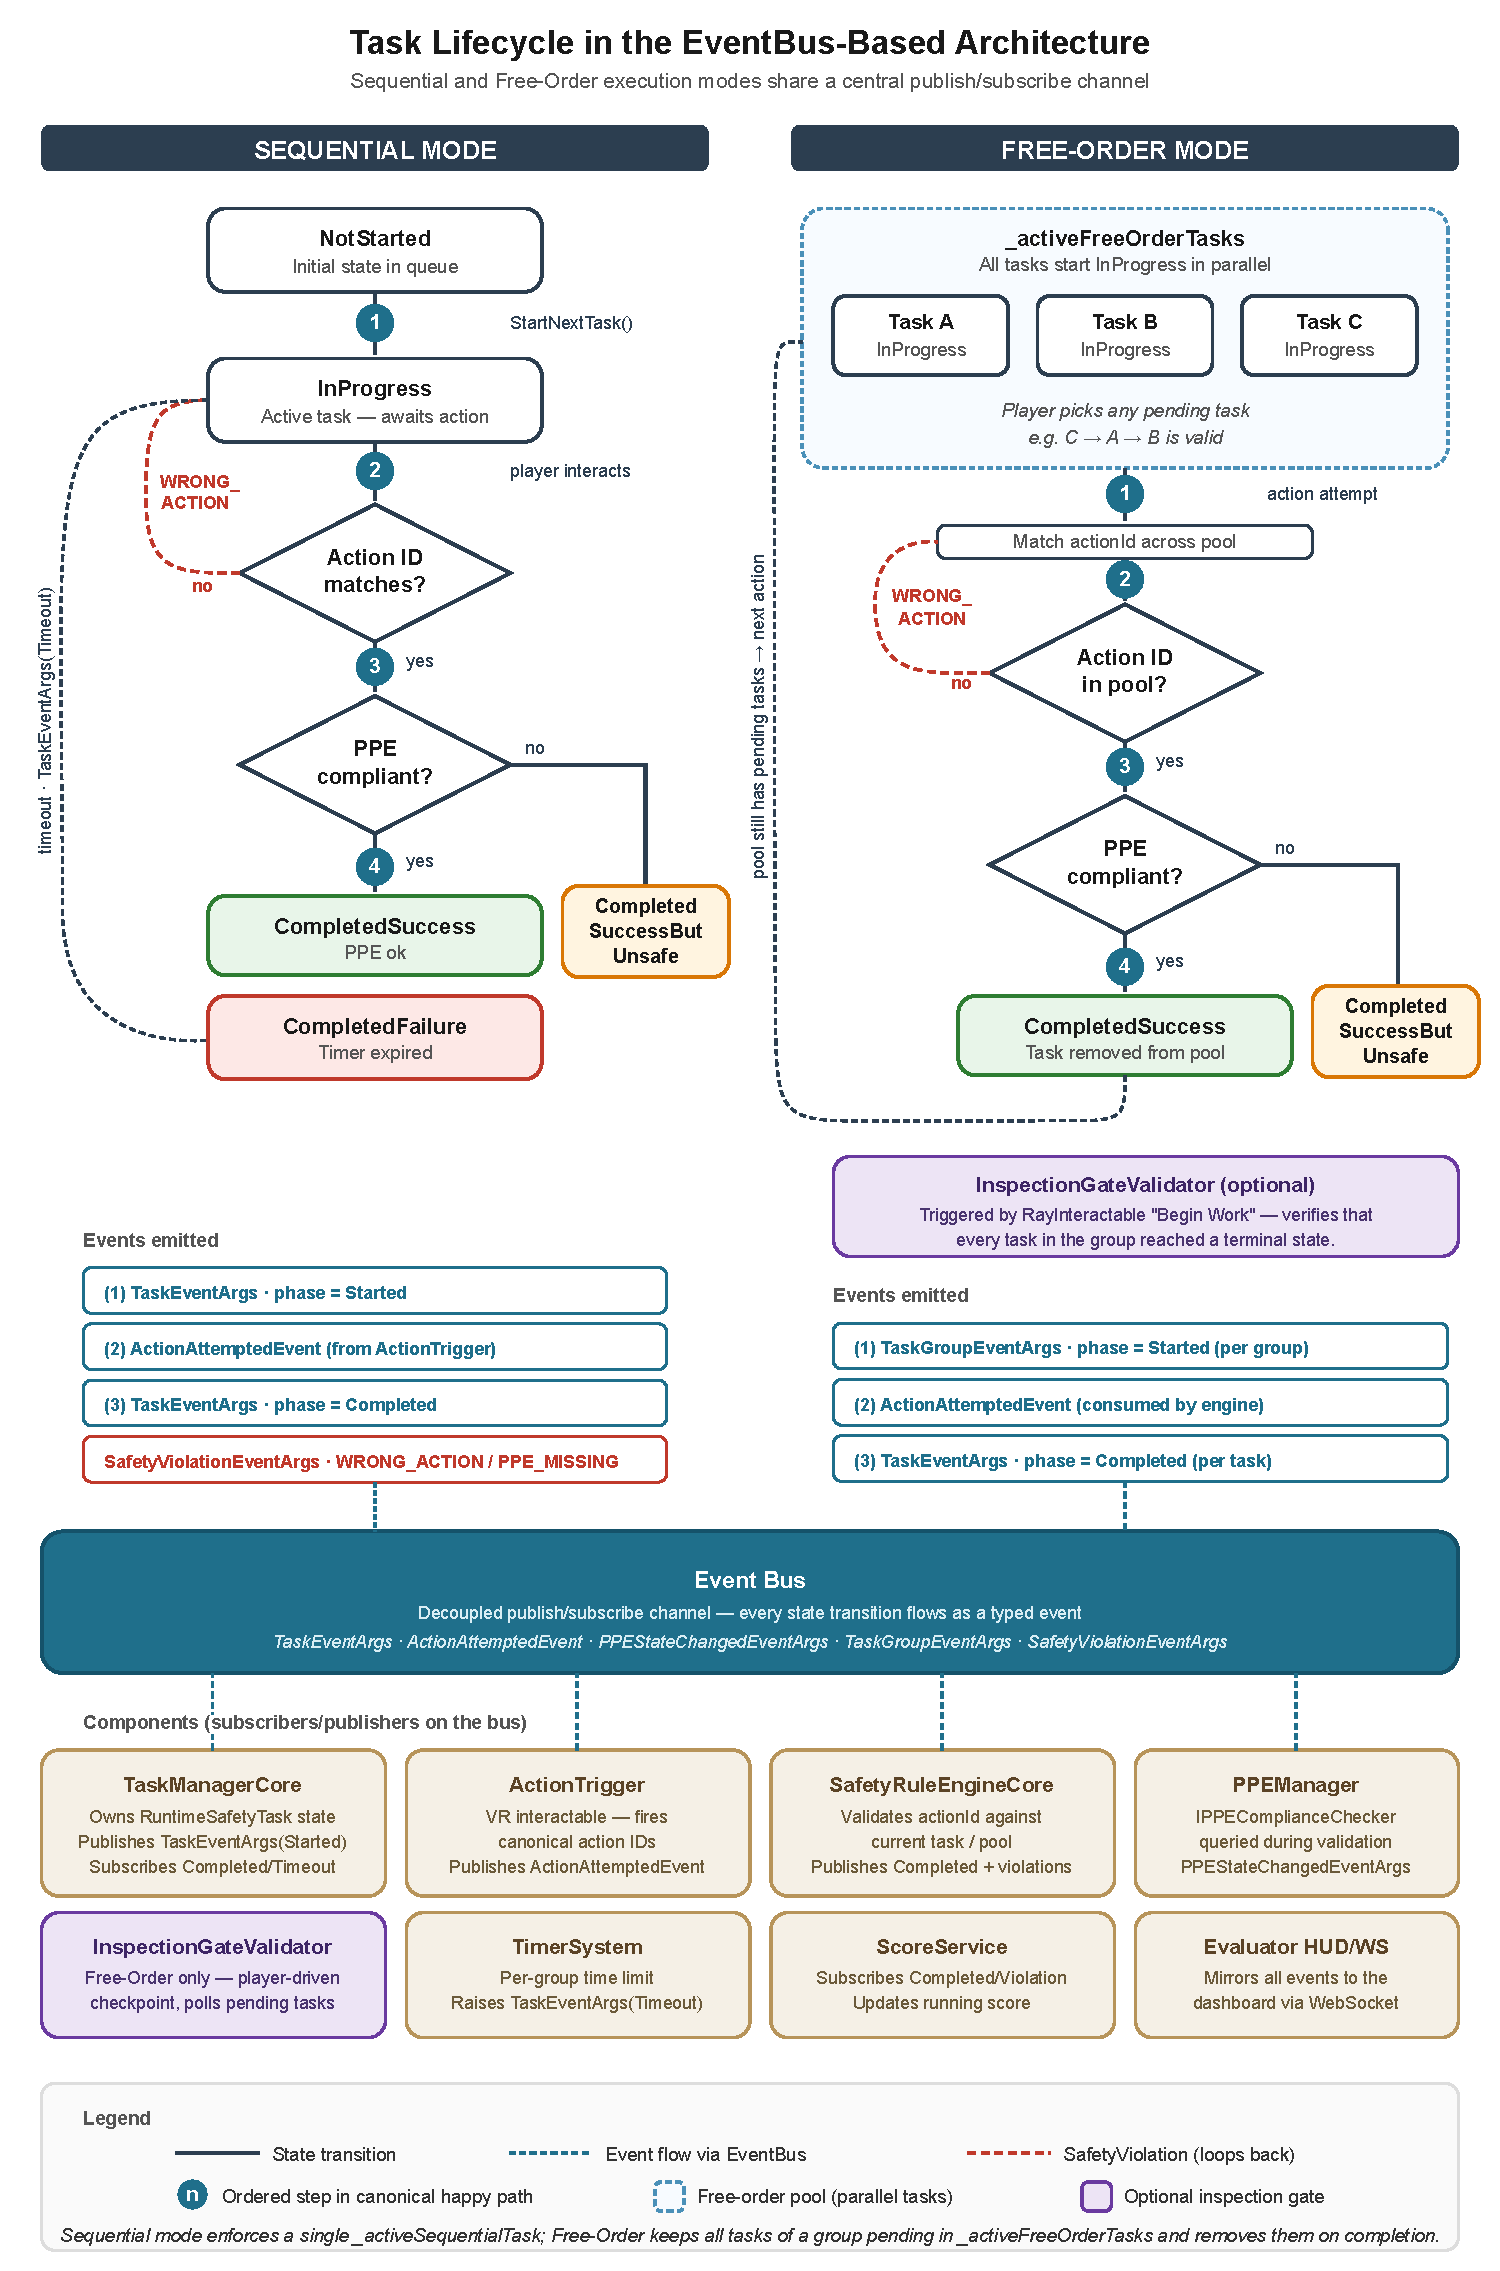
\includegraphics[width=0.85\textwidth]{figuras/task_lifecycle_vertical}

    {\footnotesize Fonte: elaborado pelo autor.}
\end{figure}

\section{Subsistema de Avaliação de Desempenho}

O subsistema de avaliação monitora, registra e analisa o desempenho dos participantes durante a execução das tarefas. Ele opera sobre o mesmo protocolo de eventos das demais camadas, o que o torna exercitável fora do motor.

\subsection{Coleta de Dados em Tempo Real}

Eventos relevantes são capturados pelo barramento à medida que ocorrem: tentativas de ação (\texttt{ActionAttempt}), conclusão ou expiração de tarefas (\texttt{TaskCompleted}, \texttt{TaskTimeout}), mudanças de estado dos EPIs (\texttt{PpeStateChanged}) e término da sessão (\texttt{SessionCompleted}). Módulos especializados interceptam esses eventos e os encaminham aos sistemas de pontuação e \textit{feedback}.

\subsection{Pontuação e Desempenho}

A avaliação quantitativa decorre de dois componentes. O \texttt{ScoreService} é um detentor de escore que expõe primitivas de mutação e notificação, mas não assina o barramento --- o que permite testá-lo isoladamente. O \texttt{ScoreRuleEngineCore} escuta os eventos de ciclo de vida das tarefas e aplica pontuação ou penalidade segundo as regras definidas nos \textit{assets} \texttt{SafetyTask}. A pontuação é atualizada em tempo real, exibida no HUD e consolidada ao final da simulação.

\subsection{Monitoramento e Exportação de Dados}

Para análise posterior, o \texttt{SessionLoggerCore} registra todos os eventos relevantes da sessão com marcação temporal e gera um arquivo \gls{JSON} com o histórico de interações e um sumário de desempenho (tempo total, tarefas concluídas, pontuação). A esse registro somam-se \textit{logs} de interação (tempo por área, número de erros, decisões tomadas) e, mediante consentimento, a gravação de vídeo da sessão para avaliação qualitativa. Os identificadores de sessão são vinculados aos dados coletados para garantir rastreabilidade entre os \textit{logs} do sistema e os questionários externos (SUS e IPQ).

\section{Racional Arquitetural}

Cinco decisões merecem justificativa.

\textbf{Eventos tipados em vez de mensagens por chave textual.} Cargas tipadas eliminam erros de execução por digitação e permitem verificação em tempo de compilação; a migração de chaves textuais resolveu três defeitos latentes de incompatibilidade entre assinantes detectados na integração.

\textbf{\texttt{ScriptableObjects} como espinha de dados.} Arquivos JSON ou XML exigiriam analisadores e ferramental próprios. Os \textit{assets} \texttt{ScriptableObject} usam o inspetor nativo, o controle de versão e a serialização do Unity, sem infraestrutura adicional.

\textbf{Acoplamento de SDK confinado às bordas.} O núcleo de domínio, o subsistema de avaliação e a interface não têm dependências do SDK. O acoplamento concentra-se nas camadas de publicadores e adaptadores, de modo que mudanças incompatíveis do SDK afetam apenas essas bordas --- o que também viabiliza substituir a entrada de RV por um leitor de console na validação técnica.

\textbf{Serialização injetada como estratégia.} O \texttt{SessionLoggerCore} recebe sua estratégia de serialização por injeção de dependência, e não embutida, permitindo implementações específicas de contexto sem modificar a lógica central.

\textbf{Despacho com orçamento de quadro.} Aplicações de RV \textit{standalone} operam sob orçamentos rígidos de CPU. O \texttt{EventBus} limita o despacho por quadro e desvia os dados de pose de alta frequência para um canal próprio, evitando que a telemetria contínua concorra com os eventos de jogo.

\section{Generalidade e Extensibilidade}

Como a lógica de domínio é independente do motor e os cenários são definidos por dados, a arquitetura oferece \textit{afordância} para múltiplos domínios de treinamento além da construção civil --- por exemplo, procedimentos clínicos, montagem industrial ou resposta a emergências. Trata-se de uma propriedade de projeto: o protótipo foi implementado e validado apenas no domínio de construção sob a NR-18 e a NR-35, e a transferência empírica para outros contextos regulatórios permanece como trabalho futuro. No mesmo sentido, um \textit{backend} distribuído poderia sustentar sessões multiusuário substituindo o \texttt{EventBus} em processo, sem alterar as camadas de aplicação.

	\chapter{Resultados Esperados}
\label{cap:resultados}

Os resultados deste trabalho são de duas naturezas. Os resultados \textbf{técnicos} já foram obtidos: dizem respeito à construção e à validação de engenharia do artefato. Os resultados \textbf{pedagógicos} são esperados e dependem da avaliação com usuários, condicionada à aprovação no Comitê de Ética em Pesquisa. Espera-se que a Fase 1 do sistema permita coletar dados preliminares relevantes sobre a eficácia do uso da Realidade Virtual (RV) como ferramenta de treinamento em segurança na construção civil, no contexto brasileiro, com foco em trabalho em altura e uso correto de EPIs.

\section{Resultados Técnicos Já Obtidos}

A construção do artefato já produziu resultados de engenharia consolidados, detalhados no Capítulo~\ref{cap:validacao}: a arquitetura orientada a eventos foi implementada e validada de forma independente do motor de jogo, com suíte de testes executada fora do Unity e confinamento das dependências de SDK às camadas de borda. Esses resultados atestam a maturidade técnica do protótipo e viabilizam a etapa de avaliação com usuários, cujos resultados, descritos a seguir, são esperados.

\section{Eficácia do Treinamento}

Espera-se que o grupo experimental demonstre ganho de conhecimento significativo sobre procedimentos de segurança em trabalho em altura e uso correto de EPIs, evidenciado pela comparação entre pré e pós-testes e superior ao do grupo controle --- indicando que a abordagem imersiva contribui de forma diferenciada em relação ao vídeo instrucional.

\section{Motivação e Engajamento}

Espera-se que o grupo experimental relate motivação e engajamento mais elevados que o grupo controle, corroborando a literatura internacional sobre a superioridade da RV frente a métodos passivos de capacitação.

\section{Qualidade da Experiência Imersiva}

Espera-se que o sistema apresente usabilidade adequada no SUS --- acima de 68 pontos, a média histórica do instrumento --- e gere presença satisfatória no IPQ junto ao grupo experimental, indicando que é usável e imersivo o suficiente para uso como ferramenta de treinamento em contexto real.

\section{Contribuição Metodológica}

Independentemente das hipóteses principais, este estudo estabelece um protocolo de avaliação adaptado ao contexto brasileiro, com grupo controle e instrumentos padronizados aplicados a trabalhadores ou estudantes da construção civil sob as NRs nacionais. Os dados fornecerão os primeiros indicadores nacionais de tamanho de efeito para esse tipo de intervenção, viabilizando o dimensionamento amostral de estudos futuros com maior poder estatístico.

\section{Sobre o Teste de Retenção}

Caso o teste de retenção caiba no cronograma, espera-se que o grupo experimental apresente maior retenção do conhecimento após 30 a 45 dias que o grupo controle, indicando que a experiência imersiva favorece a consolidação do aprendizado a longo prazo.

	\chapter{Cronograma Previsto}
\label{cap:cronograma}

A revisão bibliográfica e o desenvolvimento do protótipo encontram-se concluídos. O ambiente virtual foi implementado --- com os sistemas principais, a interface, a lógica de pontuação, o monitoramento de desempenho e o registro de eventos --- e já passou pela validação técnica descrita no Capítulo~\ref{cap:validacao}. Restam ajustes de experiência do usuário e otimização, sem alteração do fluxo de interação, já finalizado.

O tempo restante concentra-se na avaliação pedagógica com participantes, cujo caminho crítico depende de fatores externos. A defesa final tem prazo de titulação rígido em novembro de 2026. A Tabela~\ref{tab:cronograma} distribui as etapas pendentes entre junho e novembro de 2026.

\begin{table}[htb]
\centering
\caption{Cronograma das etapas restantes (2026).}
\label{tab:cronograma}
\begin{tabular}{|l|c|c|c|c|c|c|}
\hline
\textbf{Etapa} & \textbf{Jun} & \textbf{Jul} & \textbf{Ago} & \textbf{Set} & \textbf{Out} & \textbf{Nov} \\
\hline
Validação do teste de conhecimento & X & X & & & & \\
\hline
Ajustes de UX e otimização & X & X & & & & \\
\hline
Aprovação no CEP (instrumento anexado) & & X & & & & \\
\hline
Recrutamento e sessões (Camada 1) & & & X & & & \\
\hline
Teste de retenção (condicional) & & & & X & X & \\
\hline
Análise de dados & & & & & X & X \\
\hline
Redação e defesa & & & & & & X \\
\hline
\end{tabular}
\end{table}

O item de maior risco é a validação de conteúdo do teste de conhecimento, que também serve de base ao teste de retenção. Por isso, ela é prioridade imediata e corre em paralelo aos ajustes de interface. O instrumento será anexado ao protocolo do Comitê de Ética em Pesquisa antes de sua aprovação, evitando um ciclo adicional de emenda. Os questionários SUS e IPQ já estão prontos.

A coleta organiza-se em camadas, de modo que a defesa não dependa da etapa de maior incerteza de calendário. A camada primária --- ganho de conhecimento (pré e pós-teste), motivação (RIMMS), usabilidade (SUS) e presença (IPQ) --- é coletada em sessão única e ancora a avaliação. O teste de retenção, aplicado de 30 a 45 dias após o treinamento, é condicional: se não couber no prazo rígido de novembro, será declarado como limitação e recomendado para trabalho futuro, sem comprometer as demais análises.

	\chapter{Considerações Finais}
\label{cap:consideracoes}

Este projeto propõe o desenvolvimento de uma solução escalável baseada em Realidade Virtual para treinamento em segurança do trabalho no setor da construção civil. Sua principal contribuição consiste em oferecer uma alternativa tecnológica capaz de simular situações de risco de forma controlada, imersiva e repetível, com potencial para reduzir significativamente a ocorrência de acidentes em canteiros de obras. Ao capacitar os trabalhadores por meio de experiências práticas em ambientes virtuais, busca-se não apenas ampliar o conhecimento técnico, mas também promover mudanças de comportamento em relação à identificação e prevenção de riscos ocupacionais.

Entre as limitações identificadas, destaca-se o custo inicial dos equipamentos de realidade virtual imersiva, que pode restringir sua adoção por parte de empresas de pequeno e médio porte. Além disso, a implementação de tecnologias imersivas em ambientes tradicionais de formação profissional ainda demanda um processo de adaptação cultural, exigindo tempo e estratégias pedagógicas apropriadas para garantir o engajamento dos usuários.

As perspectivas futuras para o aprimoramento da proposta incluem a integração com modelos BIM (\textit{Building Information Modeling}), de forma a permitir a criação de cenários personalizados baseados em projetos reais. Também se planeja incorporar sensores e rastreadores físicos --- como \textit{trackers} acoplados aos Equipamentos de Proteção Individual (EPIs) --- para aumentar o realismo tátil da simulação e expandir os pontos de coleta de dados avaliativos. Outra frente de desenvolvimento, ainda em estágio conceitual, contempla o uso de inteligência artificial para enriquecer a atuação de um instrutor virtual, que futuramente poderá ser capaz de interagir com os participantes durante a simulação, respondendo a dúvidas sobre normas técnicas e procedimentos de segurança. Embora essa funcionalidade não esteja prevista na versão atual do sistema, trata-se de um potencial evolutivo importante, especialmente para contextos educacionais mais autônomos. Além disso, tecnologias baseadas em IA poderão ser exploradas para gerar variações dinâmicas dos cenários de simulação, evitando que os participantes decorem os roteiros e promovendo uma experiência de aprendizado mais realista e desafiadora. Por fim, espera-se estabelecer parcerias com empresas e instituições reguladoras, a fim de validar a solução em contextos reais e fomentar sua adoção como ferramenta complementar nos programas de capacitação em segurança do trabalho.


	% Elementos pós-textuais
	\bibliography{3-pos-textuais/referencias}
	\imprimiranexos
		\anexo{Roteiro da Experiência}
\label{an:roteiro}

\textbf{``Segurança no Canteiro de Obras: Prevenção de Quedas e Uso de EPIs''}

\textit{Fase 1 do Sistema Modular de Treinamento em Realidade Virtual}

\section*{1. Introdução (Cena Inicial)}

\begin{enumerate}
    \item O usuário é recebido em um canteiro de obras virtual por um instrutor virtual (engenheiro de segurança do trabalho).
    \item Breve apresentação sobre a importância das normas de segurança NR-18 e NR-35, contextualizando os riscos de trabalho em altura.
    \item Instrução sobre como interagir com o ambiente virtual: movimentação, manipulação de objetos e sistema de \textit{feedback}.
\end{enumerate}

\section*{2. Seleção de EPIs (Cena 1)}

\textbf{Cenário:} O usuário se encontra em uma área de apoio do canteiro, diante de uma bancada com diversos equipamentos, incluindo EPIs corretos e incorretos para a atividade de trabalho em altura.

\textbf{Objetivos de aprendizagem:}

\begin{itemize}
    \item Identificar os EPIs obrigatórios para trabalho em altura conforme NR-35
    \item Distinguir EPIs adequados de equipamentos inadequados ou com defeito
\end{itemize}

\textbf{Interatividade:}

\begin{enumerate}
    \item O usuário deve selecionar os EPIs corretos para a atividade que será realizada: cinto de segurança tipo paraquedista, capacete com jugular, luvas e botina de segurança.
    \item Caso selecione um EPI incorreto ou com defeito visível, o sistema fornece \textit{feedback} imediato explicando o problema.
    \item Após a seleção correta, o instrutor virtual confirma os itens escolhidos e o usuário avança para o próximo cenário já equipado.
\end{enumerate}

\textbf{Pontuação:} Acerto na seleção de cada EPI obrigatório; penalização por seleção de item inadequado.

\textbf{Mensagem educativa:} \textit{``Antes de iniciar qualquer trabalho em altura, verifique se todos os EPIs estão em bom estado e são adequados para a atividade. Nunca substitua um EPI certificado por improvisações.''}

\section*{3. Trabalho em Altura (Cena 2)}

\textbf{Cenário:} O usuário se encontra em um andaime de uma edificação em construção. O ambiente contém irregularidades deliberadas: ausência de guarda-corpo em um trecho, cinto de segurança desconectado do ponto de ancoragem e rodapé ausente em parte da plataforma.

\textbf{Objetivos de aprendizagem:}

\begin{itemize}
    \item Identificar riscos de queda em ambiente de trabalho em altura
    \item Reconhecer ausências e irregularidades em EPCs
    \item Demonstrar o procedimento correto de conexão do cinto ao ponto de ancoragem certificado
\end{itemize}

\textbf{Interatividade:}

\begin{enumerate}
    \item O usuário deve inspecionar o andaime e identificar cada irregularidade presente, interagindo com os elementos de risco.
    \item Para cada risco identificado, o usuário deve executar a correção correspondente: instalar o guarda-corpo, conectar o cinto ao ponto de ancoragem e sinalizar a ausência do rodapé.
    \item Caso o usuário tente avançar sem corrigir as irregularidades, o sistema simula a consequência do risco: animação de queda ou queda de objeto, seguida de \textit{feedback} educativo explicando o que deveria ter sido feito.
    \item Após a correção de todas as irregularidades, o instrutor virtual apresenta um resumo das boas práticas demonstradas.
\end{enumerate}

\textbf{Pontuação:} Pontos por identificação e correção de cada irregularidade; penalização por tentativa de avanço sem correção.

\textbf{Mensagem educativa:} \textit{``Em trabalhos em altura, nunca inicie a atividade sem verificar a integridade dos EPCs e a correta fixação do cinto de segurança. Um único ponto de ancoragem não verificado pode custar uma vida.''}

\section*{4. Conclusão e Avaliação Final}

\begin{enumerate}
    \item O instrutor virtual apresenta um resumo das ações realizadas pelo usuário ao longo da experiência, destacando acertos e pontos de melhoria.
    \item O usuário recebe seu relatório de desempenho gerado automaticamente pelo \textit{SessionLogger}, contendo pontuação total, tarefas concluídas e tempo de execução.
    \item O instrutor reforça as principais diretrizes das NR-18 e NR-35 aplicadas nos cenários.
    \item O usuário recebe um certificado virtual de conclusão da Fase 1 do treinamento.
\end{enumerate}

\section*{5. Nota sobre Expansão Futura}

Este roteiro corresponde à Fase 1 do sistema modular. Fases futuras preveem a incorporação de cenários adicionais como queda de objetos, escavações e contenções, e inspeção geral de canteiro, a serem desenvolvidos e validados em parceria com especialistas e entidades do setor da construção civil.

	\imprimirindice

\end{document}
